\taskpic{ Сплошной шарик подвешен в сосуде на двух одинаковых лёгких
  нитях, как показано на рисунке. Свободные концы нитей закреплены на
  одной высоте. После того как сосуд заполнили водой, и шарик оказался
  полностью погруженным в воду, натяжение нитей не изменилось.
  Определите плотность $\rho$ материала, из которого изготовлен
  шарик. Плотность воды $\rho_{\mbox{в}} = 1000\mbox{ кг/м}^3$.}
{
  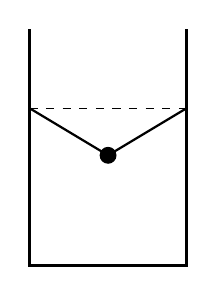
\begin{tikzpicture}
    \draw[very thick] (0,3) -- (0,0) -- (2,0) -- (2,3);
    \draw[dashed] (0,2) -- (2,2);
    \draw[thick] (0,2) -- (1,1.4) -- (2,2);
    \draw[fill=black] (1,1.4) circle (0.1cm);
  \end{tikzpicture}
}
% Московская городская олимпиада, 2007